\documentclass[12pt]{article}

\usepackage[utf8]{inputenc}
\usepackage{amssymb}
\usepackage[brazilian]{babel}
\usepackage{graphicx}
\usepackage { anysize } 
\begin{document}

\title{Redução de Dimensionalidade usando uma modificação do algoritmo Autofaces Fracionário}
\author{Emanuel D. Ferreira dos Santos, Tiago Buarque de Carvalho}
\maketitle

\abstract{\noindent
Este trabalho visa expor os resultados da modificação do algoritmo Autofaces Fracionário. O método proposto funciona substituindo o parâmetro escalar $r$, por um vetor de tamanho variável $R$. A fim de encontrar os valores do vetor $R$ que maximizassem o valor da acurácia, escolhemos usar um Algoritmo Genético como meta-heurística capaz de nos fornecer esse resultado. Nos experimentos, comparamos o método proposto com o Autofaces Fracionário, aplicando ambos em seis bases de dados reais e calculando métricas de avaliação usando o classificador 1-NN.
\\
\\
\noindent
\textbf{palavras-chave}: redução de dimensionalidade, PCA, Algoritmo Genético, Autofaces Fracionário.
}

\section{Introdução}

No contexto de redução de dimensionalidade, o termo \textit{dimensionalidade} se refere a quantidade de variáveis aleatórias que um determinado conjunto de dados possui. Assim, se uma amostra $x\textsubscript{i}$ é definida por

$$
x_i = [\alpha_1 ,\alpha_2 ,\ldots,\alpha_n],
$$

dizemos que a amostra $x_i$ possui dimensionalidade $n$, sendo que $n \in \mathbb{N}\textsuperscript{*} $.\linebreak
\indent A redução de dimensionalidade acontece quando conseguimos diminuir o número de atributos do conjunto original de modo que ainda tenhamos uma versão que seja representativa dos dados originais.\linebreak
\indent Para o Aprendizado de Máquina, a importância da redução de dimensionalidade consiste em poder submeter para os algoritmos apenas os atributos que sejam mais relevantes no que se refere ao manuseio dos dados.

\section{Algoritmos Relacionados}

Muitos métodos têm sido propostos a fim de melhorar a qualidade dos algoritmos de redução de dimensionalidade. Alguns deles derivam do método algébrico PCA, o qual é conhecido como o mais bem estabelecido na literatura. Nessa secção falaremos sobre o funcionamento do PCA e três métodos derivados dele: FPCA, Autofaces e Autofaces Fracionário.

\subsection{PCA}

PCA (Principal Component Analysis, em português Análise dos Componentes Principais) é  uma técnica de redução de dimensionalidade que ao receber como entrada um dataset $D$ com dimensão $m$, produz uma projeção de $D$ no espaço de dimensionalidade $m'$, sendo $m' < m$.

Seja $D$ uma matriz que contém os dados a serem reduzidos. Temos que a matriz $D$, contendo $n$ amostras é definida como

$$
D = \left[
\begin{array}{l}
x_1\\
x_2\\
x_3\\
\vdots\\
x_n
\end{array}
\right]
$$

Cada amostra $x_i$ contém $m$ varíáveis, as quais chamamos de atributos. Desta forma temos

$$
x_i = \left[
\begin{array}{cccc}
x_{i1}, &
x_{i2}, &
..., &
x_{im}
\end{array}
\right]
$$

O vetor médio $\overline{x}$ é do conjunto de dados é obtido através da fórmula \ref{eq:media}.

\begin{equation}
\overline{x} = \frac{1}{n} \Sigma x_j \label{eq:media}
\end{equation}

Subtraindo o vetor médio de cada amostra de $D$, teremos uma versão do dados centralizada na origem:

$$
D' = \left[
\begin{array}{l}
(x_1 - \overline{x})\\
(x_2 - \overline{x})\\
(x_3 - \overline{x})\\
\vdots\\
(x_n - \overline{x})
\end{array}
\right]
$$

A partir de $D'$ é possível obter a matriz de covariância dos dados. Essa matriz contém o valor da covariância entre cada par de atributos, bem como a variância de cada atributo na diagonal principal. Ela pode ser obtida através de

\begin{equation}
Cov(D') = \frac{1}{n} D'\textsuperscript{T} D' \label{eq:cov_mat}
\end{equation}

A matriz $Cov(D')$ será de ordem $m x m$.

Cada coluna da matriz $Cov(D')$ é uma autovetor. Dessa forma temos que


$$
Cov(D') = [\xi_1, \xi_2, ..., \xi_m]
$$

Onde para cada autovetor $\xi_i$ existe um autovelor $\lambda_i$ associado, o qual representa a variância daquele atributo.

NÂO CONCLUIDO

\subsection{PCA Fracionário}

Lorem ipsum dolor sit amet, consectetur adipiscing elit. Praesent porta, lorem non faucibus condimentum, orci orci condimentum lectus, sit amet sollicitudin justo libero non dui. Sed sollicitudin leo at urna dapibus cursus. Vestibulum nibh dui, tristique vitae mollis tristique, sagittis pretium justo. Nulla faucibus suscipit dolor eu semper. Nam nisl lacus, tempor quis nisi vitae, dictum sollicitudin dolor. Vivamus quis elit consequat, ullamcorper ligula non, ultricies enim. Proin dictum leo eget tempor placerat. Cras dapibus eget lorem sed malesuada. Mauris lobortis iaculis purus, eu varius neque lacinia et. Vivamus gravida nisl in pellentesque molestie. Aliquam sit amet urna ut nulla faucibus eleifend sit amet sed nibh. Nam porta leo sed enim interdum posuere. Duis purus diam, volutpat vel luctus sit amet, venenatis at lacus. 

\subsection{Autofaces}

Lorem ipsum dolor sit amet, consectetur adipiscing elit. Praesent porta, lorem non faucibus condimentum, orci orci condimentum lectus, sit amet sollicitudin justo libero non dui. Sed sollicitudin leo at urna dapibus cursus. Vestibulum nibh dui, tristique vitae mollis tristique, sagittis pretium justo. Nulla faucibus suscipit dolor eu semper. Nam nisl lacus, tempor quis nisi vitae, dictum sollicitudin dolor. Vivamus quis elit consequat, ullamcorper ligula non, ultricies enim. Proin dictum leo eget tempor placerat. Cras dapibus eget lorem sed malesuada. Mauris lobortis iaculis purus, eu varius neque lacinia et. Vivamus gravida nisl in pellentesque molestie. Aliquam sit amet urna ut nulla faucibus eleifend sit amet sed nibh. Nam porta leo sed enim interdum posuere. Duis purus diam, volutpat vel luctus sit amet, venenatis at lacus. 

\subsection{Autofaces Fracionário}

Lorem ipsum dolor sit amet, consectetur adipiscing elit. Praesent porta, lorem non faucibus condimentum, orci orci condimentum lectus, sit amet sollicitudin justo libero non dui. Sed sollicitudin leo at urna dapibus cursus. Vestibulum nibh dui, tristique vitae mollis tristique, sagittis pretium justo. Nulla faucibus suscipit dolor eu semper. Nam nisl lacus, tempor quis nisi vitae, dictum sollicitudin dolor. Vivamus quis elit consequat, ullamcorper ligula non, ultricies enim. Proin dictum leo eget tempor placerat. Cras dapibus eget lorem sed malesuada. Mauris lobortis iaculis purus, eu varius neque lacinia et. Vivamus gravida nisl in pellentesque molestie. Aliquam sit amet urna ut nulla faucibus eleifend sit amet sed nibh. Nam porta leo sed enim interdum posuere. Duis purus diam, volutpat vel luctus sit amet, venenatis at lacus.

\section{Algoritmo Genético}

Lorem ipsum dolor sit amet, consectetur adipiscing elit. Praesent porta, lorem non faucibus condimentum, orci orci condimentum lectus, sit amet sollicitudin justo libero non dui. Sed sollicitudin leo at urna dapibus cursus. Vestibulum nibh dui, tristique vitae mollis tristique, sagittis pretium justo. Nulla faucibus suscipit dolor eu semper. Nam nisl lacus, tempor quis nisi vitae, dictum sollicitudin dolor. Vivamus quis elit consequat, ullamcorper ligula non, ultricies enim. Proin dictum leo eget tempor placerat. Cras dapibus eget lorem sed malesuada. Mauris lobortis iaculis purus, eu varius neque lacinia et. Vivamus gravida nisl in pellentesque molestie. Aliquam sit amet urna ut nulla faucibus eleifend sit amet sed nibh. Nam porta leo sed enim interdum posuere. Duis purus diam, volutpat vel luctus sit amet, venenatis at lacus.  

\section{Método Proposto}

O método proposto consiste em modificar o Autoface Fracionário por meio da aplicação de um vetor $R$ no lugar da escalar $r$. Cada elemento de $R$ seria aplicado sobre uma fração da amostra. Para o caso específico de imagens, um vetor $R$ de comprimento $n$ implicaria que a amostra seria dividida em uma matriz $\sqrt{n}x\sqrt{n}$. Assim teríamos uma variação maior do parâmetro $r$ original do Autofaces Fracionário sobre a amostra de entrada.\newline
\indent
Para a obtenção do vetor $R$, foi usado um Algoritmo Genético com o objetivo de se conseguir bons valores para o vetor e que por consequência melhorasse a qualidade da redução de dimensionalidade e por conseguinte a acurácia do algoritmo de classificação utilizado.
\section{Experimentos}

Datasets adotados nos experimentos podem ser conferidos na Tabela 1.

\begin{table}[] \centering
\scriptsize
\begin{tabular}{|l|l|l|l|}
\hline
\textbf{Base} & \multicolumn{1}{r|}{\textbf{Nº de amostras}} & \textbf{N º de atributos} & \textbf{Nº de classes} \\ \hline
Yale Faces       & 10212                                        & 12123                     & 10                     \\ \hline
Sheffield        & 12323                                        & 12323                     & 12                     \\ \hline
AT\&T            & 12323                                        & 1223                      & 12                     \\ \hline
Georgia Tech     & 123232                                       & 123213                    & 123                    \\ \hline
Faces 95         & 2123123                                      & 1212323                   & 12323                  \\ \hline
AR               & 123232                                       & 232323                    & 23                     \\ \hline
FEI               & 123232                                       & 232323                    & 23                     \\ \hline
\end{tabular}
\caption{Bases de dados utilizadas nos experimentos.}
\end{table}

\subsection{Metodologia Adotada}
A metodologia dos experimentos realizados para calcular os valores do vetor $R$ pode ser conferida no fluxograma da Figura \ref{fig:diagrama1}. Após a obtenção do vetor $R$, uma outro algoritmo é executado a fim de comparar os desempenhos do Autofaces Fracionário e do Autofaces Fracionário proposto. Esse algoritmo pode ser observado na Figura \ref{fig:diagrama2}.\\
\indent Os valores de componentes testados em cada execução do Algoritmo Genético foram os seguintes:

$$c = [1, 5, 10, 15, 20, 25, 30, 35, 40, 45, 50, 55, 60, 65, 70]$$

Assim, cada experimento executou um Algoritmo Genético 15 vezes, uma para cada número de componentes. Além disso, cada execução do AG resultava em um vetor R para algum número de componentes considerado no momento.

\begin{figure}[!h] \centering
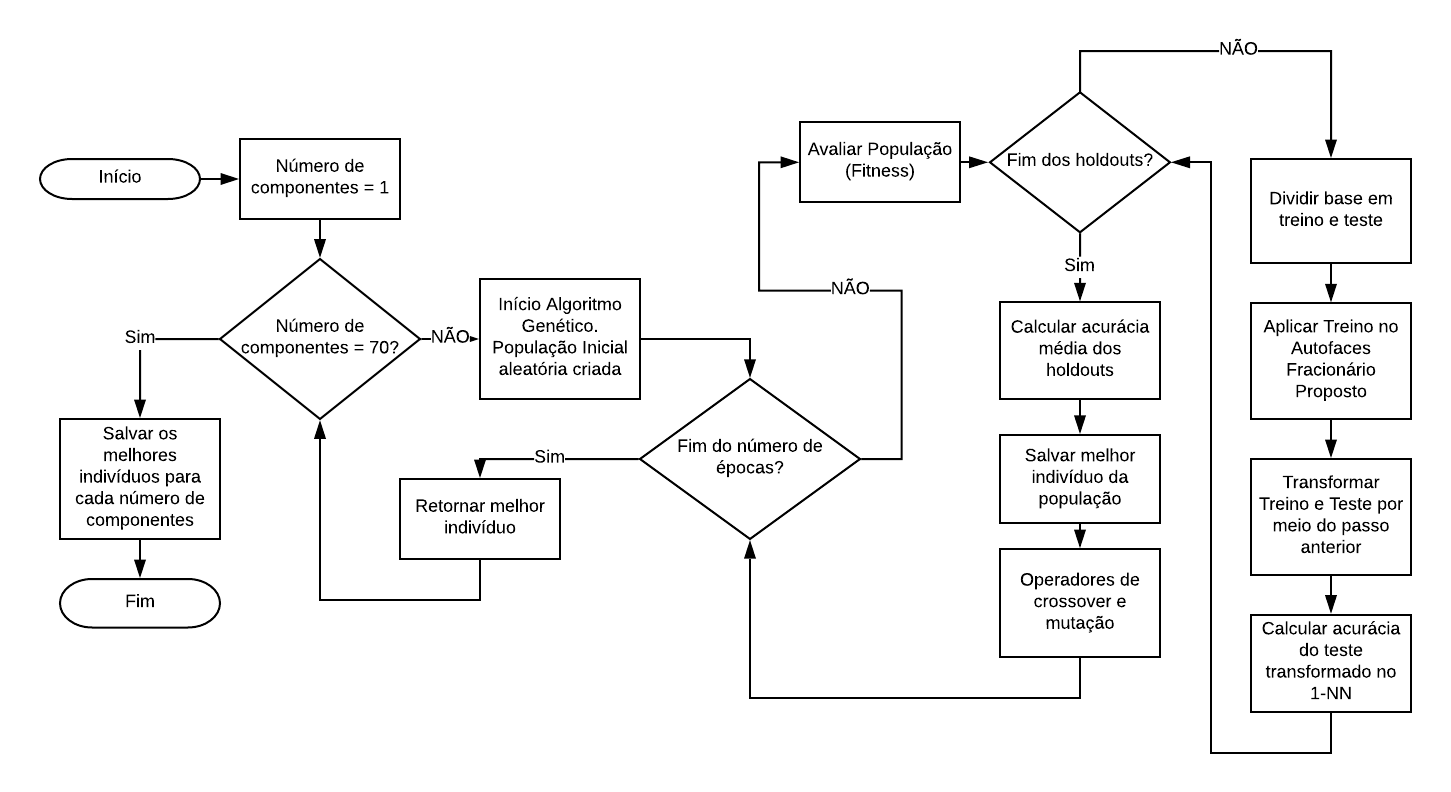
\includegraphics[scale=0.7]{diagrama1.png}
\caption{Digrama do algoritmo genético utilizado para obter valores de $R$.}
\label{fig:diagrama1}
\end{figure}

\begin{figure}[!h] \centering
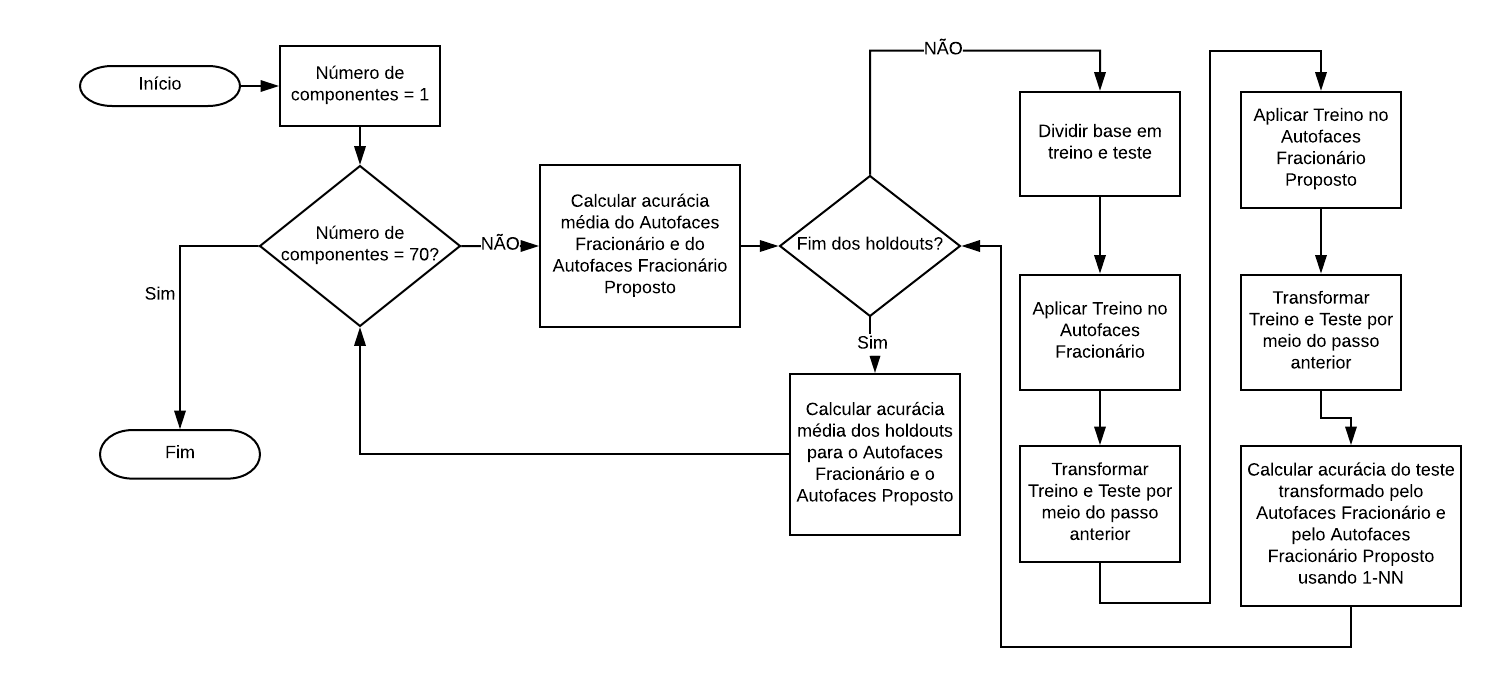
\includegraphics[scale=0.7]{diagrama2.png}
\caption{Digrama do algoritmo que compara o desempenho entre o Autofaces Fracionário e o proposto.}
\label{fig:diagrama2}
\end{figure}

\subsection{Resultados}

Lorem ipsum dolor sit amet, consectetur adipiscing elit. Praesent porta, lorem non faucibus condimentum, orci orci condimentum lectus, sit amet sollicitudin justo libero non dui. Resultados podem ser vistos nos gráficos da Figura \ref{fig:Res}

\begin{figure}[!h] \centering 
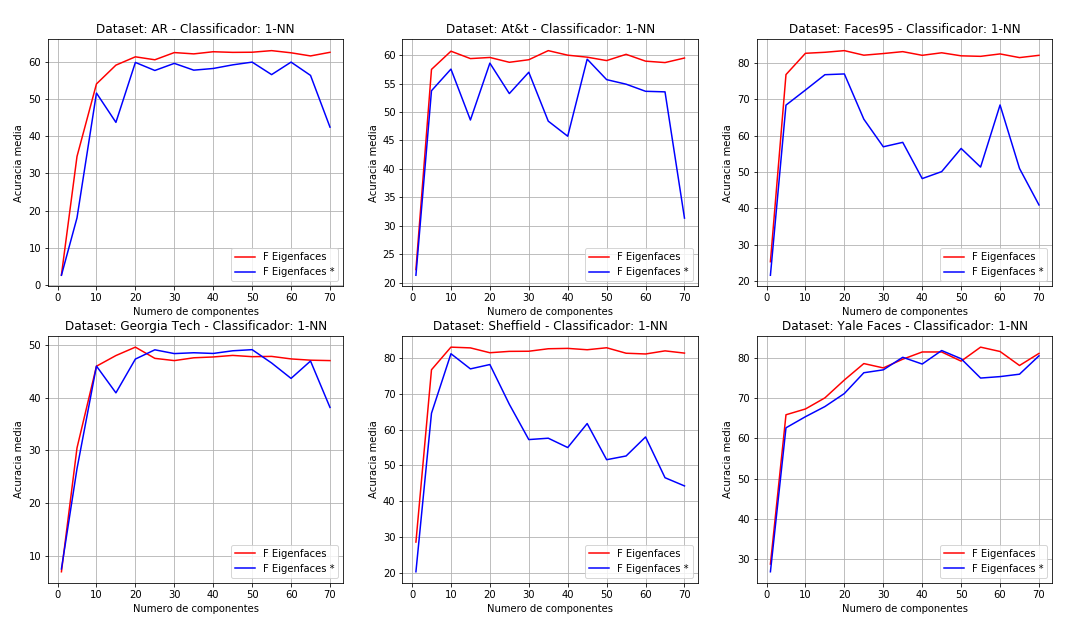
\includegraphics[scale=0.5]{resultados.png}
\caption{Resultados para os seis datasets} 
\label{fig:Res} \end{figure} 

\section{Conclusões}

Lorem ipsum dolor sit amet, consectetur adipiscing elit. Praesent porta, lorem non faucibus condimentum, orci orci condimentum lectus, sit amet sollicitudin justo libero non dui. Sed sollicitudin leo at urna dapibus cursus. Vestibulum nibh dui, tristique vitae mollis tristique, sagittis pretium justo. Nulla faucibus suscipit dolor eu semper. Nam nisl lacus, tempor quis nisi vitae, dictum sollicitudin dolor. Vivamus quis elit consequat, ullamcorper ligula non, ultricies enim. Proin dictum leo eget tempor placerat. Cras dapibus eget lorem sed malesuada. Mauris lobortis iaculis purus, eu varius neque lacinia et. Vivamus gravida nisl in pellentesque molestie. Aliquam sit amet urna ut nulla faucibus eleifend sit amet sed nibh. Nam porta leo sed enim interdum posuere. Duis purus diam, volutpat vel luctus sit amet, venenatis at lacus. 

\section{Referências}

Lorem ipsum dolor sit amet, consectetur adipiscing elit. Praesent porta, lorem non faucibus condimentum, orci orci condimentum lectus, sit amet sollicitudin justo libero non dui. Sed sollicitudin leo at urna dapibus cursus. Vestibulum nibh dui, tristique vitae mollis tristique, sagittis pretium justo. Nulla faucibus suscipit dolor eu semper. Nam nisl lacus, tempor quis nisi vitae, dictum sollicitudin dolor. Vivamus quis elit consequat, ullamcorper ligula non, ultricies enim. Proin dictum leo eget tempor placerat. Cras dapibus eget lorem sed malesuada. Mauris lobortis iaculis purus, eu varius neque lacinia et. Vivamus gravida nisl in pellentesque molestie. Aliquam sit amet urna ut nulla faucibus eleifend sit amet sed nibh. Nam porta leo sed enim interdum posuere. Duis purus diam, volutpat vel luctus sit amet, venenatis at lacus. 



\end{document}

